% ReRoom -- differentiable proximal projection Pi_theta (paper-figure style).
\documentclass[border=6pt]{standalone}
\usepackage{tikz}\usepackage{amsmath,amssymb}
\usetikzlibrary{arrows.meta,positioning,calc}
\definecolor{ink}{HTML}{1A1A1A}\definecolor{mut}{HTML}{6B7280}
\definecolor{net}{HTML}{3B5BD9}\definecolor{prj}{HTML}{E8770F}
\tikzset{
  slbl/.style={font=\tiny,text=mut},
  it/.style ={draw=ink,line width=.7pt,circle,fill=white,inner sep=1.5pt,font=\small},
  a/.style  ={-{Stealth[length=4.5pt]},line width=.8pt,ink},
  wall/.style={line width=.7pt,ink},
}
\newcommand{\furn}[5]{\fill[#5,rounded corners=.3pt] (#1,#2) rectangle ++(#3,#4);}
\begin{document}
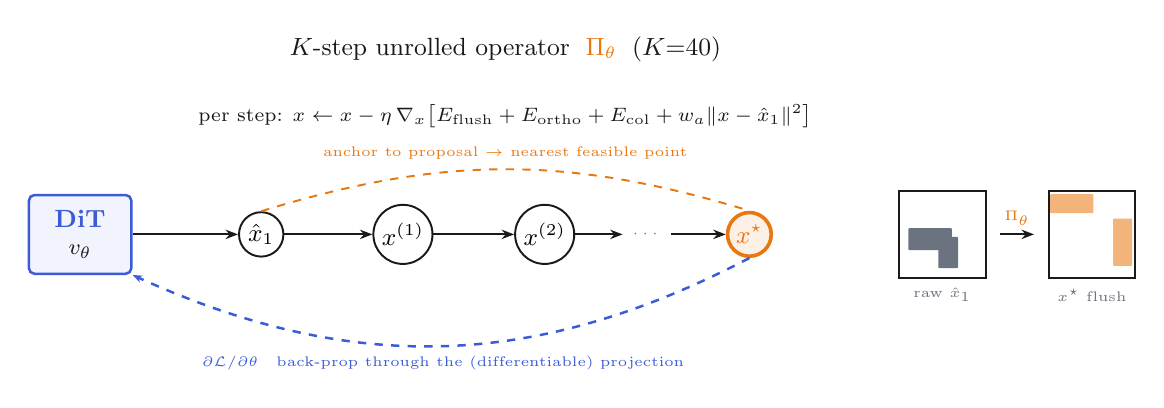
\begin{tikzpicture}
% DiT source
\node[draw=net,line width=.9pt,rounded corners=2pt,fill=net!7,minimum width=13mm,minimum height=10mm,align=center,font=\small,text=ink] (dit) at (0,0) {\textbf{\textcolor{net}{DiT}}\\[-1pt]{\footnotesize $v_\theta$}};
% iteration chain
\node[it] (x0) at (2.3,0) {$\hat x_1$};
\node[it] (x1) at (4.1,0) {$x^{(1)}$};
\node[it] (x2) at (5.9,0) {$x^{(2)}$};
\node[slbl] (dots) at (7.2,0) {$\cdots$};
\node[it,draw=prj,line width=1.3pt,fill=prj!10,text=prj] (xs) at (8.5,0) {$x^{\star}$};
\draw[a] (dit) -- (x0);
\draw[a] (x0) -- (x1); \draw[a] (x1) -- (x2); \draw[a] (x2) -- (dots); \draw[a] (dots) -- (xs);
% title
\node[font=\small,text=ink] at (5.4,2.35) {$K$-step unrolled operator \;\textbf{\textcolor{prj}{$\Pi_\theta$}}\; ($K{=}40$)};
% anchor arc (above)
\draw[prj,dashed,line width=.7pt] (x0.north) to[bend left=17] node[above,slbl,text=prj,pos=.5]{anchor to proposal $\to$ nearest feasible point} (xs.north);
% per-step update (above the chain)
\node[font=\scriptsize,text=ink] at (5.4,1.5) {per step: $x\leftarrow x-\eta\,\nabla_x\!\left[E_\text{flush}+E_\text{ortho}+E_\text{col}+w_a\lVert x-\hat x_1\rVert^2\right]$};
% back-prop arc (below, to DiT)
\draw[net,dashed,line width=.9pt,-{Stealth[length=3.5pt]}] (xs.south) to[bend left=26] node[below,slbl,text=net,pos=.5]{$\partial\mathcal{L}/\partial\theta$ \; back-prop through the (differentiable) projection} (dit.south east);
% before -> after room snap (right)
\begin{scope}[shift={(10.4,-0.55)}]
  \draw[wall] (0,0) rectangle (1.1,1.1);
  \furn{0.12}{0.35}{0.55}{0.28}{mut}\furn{0.5}{0.12}{0.25}{0.4}{mut}
  \node[slbl] at (0.55,-0.22){raw $\hat x_1$};
  \draw[a,shorten >=1pt,shorten <=1pt] (1.25,0.55) -- (1.75,0.55);
  \node[slbl,prj] at (1.5,0.75){$\Pi_\theta$};
  \draw[wall] (1.9,0) rectangle (3.0,1.1);
  \furn{1.92}{0.82}{0.55}{0.24}{prj!55}\furn{2.72}{0.15}{0.24}{0.6}{prj!55}
  \node[slbl] at (2.45,-0.22){$x^{\star}$ flush};
\end{scope}
\end{tikzpicture}
\end{document}
